%15 min preso!
\documentclass[xcolor=table,aspectratio=169]{beamer}
\usepackage{beamerthemesplit}
\usepackage{wrapfig}
\usetheme{SPbGU}
\usepackage{pdfpages}
\usepackage{amsmath}
\usepackage{cmap}
\usepackage[T2A]{fontenc}
\usepackage[utf8]{inputenc}
\usepackage[english]{babel}
\usepackage{indentfirst}
\usepackage{amsmath}
\usepackage{tikz}
\usepackage{multirow}
\usepackage[noend]{algpseudocode}
\usepackage{algorithm}
\usepackage{algorithmicx}
\usepackage{fancyvrb}
\usepackage{hyperref} 
\definecolor{links}{HTML}{2A1B81}
\hypersetup{colorlinks,linkcolor=,urlcolor=links}
\usetikzlibrary{calc}
\usetikzlibrary{shapes, backgrounds}
\usetikzlibrary{arrows,automata}
\usetikzlibrary{positioning}
\usetikzlibrary{fit}
\usetikzlibrary{shapes.callouts}
\usetikzlibrary{shapes.misc}
\usepackage{xparse}
\usepackage{fontawesome}

\usepackage{etoolbox,refcount}
\usepackage{multicol}

\usepackage{tabularx}
\newcolumntype{Y}{>{\raggedleft\arraybackslash}X}

\renewcommand{\thealgorithm}{}

\newtheorem{mytheorem}{Theorem}
\renewcommand{\thealgorithm}{}

\newcommand{\tikzmark}[1]{\tikz[overlay,remember picture] \node (#1) {};}
\def\Put(#1,#2)#3{\leavevmode\makebox(0,0){\put(#1,#2){#3}}}

\newcommand{\ltz}{$< 1$}
\definecolor{Gray}{gray}{0.8}

\tikzset{
    state/.style={
           rectangle,
           rounded corners,
           draw=black, very thick,
           minimum height=2em,
           inner sep=2pt,
           text centered,
           },
}

\tikzset{
    invisible/.style={opacity=0,text opacity=0},
    visible on/.style={alt=#1{}{invisible}},
    alt/.code args={<#1>#2#3}{%
      \alt<#1>{\pgfkeysalso{#2}}{\pgfkeysalso{#3}} % \pgfkeysalso doesn't change the path
    },
}

\tikzset{cross/.style={cross out, draw=black, minimum size=2*(#1-\pgflinewidth), inner sep=0pt, outer sep=0pt, ultra thick},
%default radius will be 1pt. 
cross/.default={1pt}}

\NewDocumentCommand{\mycallout}{r<> O{opacity=0.8,text opacity=1} m m m}{%
\tikz[remember picture, overlay]\node[align=center, fill=cyan!20, text width=#5cm,
#2,visible on=<#1>, rounded corners,
draw,rectangle callout,anchor=pointer,callout relative pointer={(290:0.5cm)}]
at (#3) {#4};
}

\NewDocumentCommand{\mycalloutR}{r<> O{opacity=0.8,text opacity=1} m m m}{%
\tikz[remember picture, overlay]\node[align=center, fill=cyan!20, text width=#5cm,
#2,visible on=<#1>, rounded corners,
draw,rectangle callout,anchor=pointer,callout relative pointer={(30:0.8cm)}]
at (#3) {#4};
}

\newcommand\colR{\cellcolor{red!20}}
\newcommand\colB{\cellcolor{blue!20}}
\newcommand\colG{\cellcolor{green!20}}

%callout relative pointer={(230:0.5cm)}]

\newcounter{countitems}
\newcounter{nextitemizecount}
\newcommand{\setupcountitems}{%
  \stepcounter{nextitemizecount}%
  \setcounter{countitems}{0}%
  \preto\item{\stepcounter{countitems}}%
}
\makeatletter
\newcommand{\computecountitems}{%
  \edef\@currentlabel{\number\c@countitems}%
  \label{countitems@\number\numexpr\value{nextitemizecount}-1\relax}%
}
\newcommand{\nextitemizecount}{%
  \getrefnumber{countitems@\number\c@nextitemizecount}%
}
\newcommand{\previtemizecount}{%
  \getrefnumber{countitems@\number\numexpr\value{nextitemizecount}-1\relax}%
}
\makeatother    
\newenvironment{AutoMultiColItemize}{%
\ifnumcomp{\nextitemizecount}{>}{3}{\begin{multicols}{2}}{}%
\setupcountitems\begin{itemize}}%
{\end{itemize}%
\unskip\computecountitems\ifnumcomp{\previtemizecount}{>}{3}{\end{multicols}}{}}

\setbeamertemplate{page number in head/foot}[appendixframenumber]
\setbeamertemplate{itemize item}[circle]
\setbeamertemplate{itemize subitem}[smallblacktriangleright]

\beamertemplatenavigationsymbolsempty

\title[GraphBLAS: проблемы и перспективы]{Обобщённая разреженная линейная алгебра и высокопроизводительный анализ графов: проблемы и перспективы}
\subtitle{Graph Analytics Club}
\institute[СПбГУ]{
Санкт-Петербургский Государственный Университет
}

% То, что в квадратных скобках, отображается в левом нижнем углу.
\author[Семён Григорьев]{Семён Григорьев}

\date{10 сентября 2025}

\begin{document}
{
\begin{frame}[fragile]
  \begin{table}
  \centering
  %
\includegraphics[height=1.5cm]{pictures/SPbGU_Logo.png}
  \begin{tabularx}{\linewidth}{XcX}
    
\includegraphics[height=1.3cm]{pictures/GAC_logo.jpg} 
    \hfill
    & 
    & \hfill 
\includegraphics[height=1.6cm]{pictures/SPbGU_Logo.png}
  \end{tabularx}
  \end{table}
  \titlepage
\end{frame}
}

\begin{frame}[fragile]
  \frametitle{Семён Григорьев}
  \begin{minipage}{0.70\textwidth}
  \begin{itemize}    
    \item Доцент кафедры системного программирования Санкт-Петербургского Государственного Университета
    %\item Научный сотрудник лаборатории YADRO
    \item Руководитель исследовательской группы
    \item Области интересов
    \begin{itemize}
      \item \textbf{Высокопроизводительная линейная алгебра} для анализа графов
      \begin{itemize}
        \item \textbf{Обобщённая}: матрицы и вектора параметризованы типом элемента, операции над ними могут быть заданы пользователем
        \item \textbf{Разреженная}: специализированные структуры для хранения матриц и векторов, специализированные алгоритмы для их обработки 
        \item В том числе, с использованием \textbf{графических ускорителей}
      \end{itemize}
      \item \textbf{Высокопроизводительный анализ графов}      
    \end{itemize}
    \end{itemize}
\end{minipage}
\begin{minipage}[t]{0.29\textwidth}
  \begin{center}
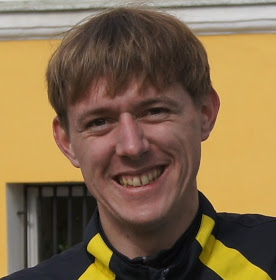
\includegraphics[width=0.8\textwidth]{pictures/SemyonGrigorev.jpg}
  \end{center}
  {\scriptsize
\begin{itemize}    
  \item Email: s.v.grigoriev@mail.spbu.ru
  \item GitHub: \href{https://github.com/gsvgit}{gsvgit}
  \item Google Scholar: \href{https://scholar.google.com/citations?hl=ru&user=kP4dqUAAAAAJ&view_op=list_works&sortby=pubdate}{Semyon Grigorev}
  \item DBLP: \href{https://dblp.org/pid/181/9903.html}{Semyon V. Grigorev}
\end{itemize}
  }
\end{minipage}
\end{frame}

\begin{frame}[fragile]
  \begin{center}\huge
    Как создать <<достаточно универсальный>> фреймворк для разработки высокопроизводительных (параллельных) алгоритмов анализа графов?
  \end{center}
\end{frame}


\begin{frame}[fragile]
  \frametitle{GraphBLAS\footnote{\url{https://graphblas.org/}}}
  \begin{itemize}
    \item API для создания алгоритмов анализа графов на основе линейной алгебры 
    \begin{itemize}
      \item Различные операции над матрицами и векторами (\underline{\textbf{разреженными}})
      \item Параметризация алгебраическими структурами: полукольцами, моноидами и т.д.
    \end{itemize}
    \item Позволяет выражать \underline{\textbf{различные}} алгоритмы
    \begin{itemize}
      \item Обход в ширину, поиск кратчайших путей, достижимость, \ldots
      \item Подсчёт треугольников, PageRank, остовные деревья, кластеризация, \ldots
      \item[\color{red}{\tiny{$\blacktriangleright$}}] Навигационные запросы: \textbf{RPQ, CFPQ,} \ldots
    \end{itemize}
    \item Подробнее
    \begin{itemize}
      \item The GraphBLAS C API Specification\footnote{\url{https://graphblas.org/docs/GraphBLAS_API_C_v2.1.0.pdf}}
      \item GraphBLAS Pointers\footnote{\url{https://graphblas.org/GraphBLAS-Pointers/}}
      \item Introduction to GraphBLAS\footnote{\url{https://zenodo.org/record/4318870/files/graphblas-introduction.pdf}}
      \item LAGraph\footnote{\url{https://github.com/GraphBLAS/LAGraph}}
    \end{itemize}
    \end{itemize}
\end{frame}

\begin{frame}[fragile]
  \frametitle{Реализации GraphBLAS-подобных API}
  \begin{itemize}
      \item \textbf{SuiteSparse:GraphBLAS}\footnote{\url{https://github.com/DrTimothyAldenDavis/GraphBLAS}} --- \underline{\textbf{эталон}} на чистом C\footnote{Ведётся работа над использованием GPGPU через Cuda} (Intel, Nvidia)
      \item Huawei's GraphBLAS\footnote{\url{https://gitee.com/CSL-ALP/graphblas}} --- частичная реализация на C++
      \item CombBLAS\footnote{\url{https://github.com/PASSIONLab/CombBLAS}} --- распределённая, частичная реализация на C++
      \item GraphBLAST\footnote{\url{https://github.com/gunrock/graphblast}} --- поддержка GPGPU, Cuda C, частичная реализация
      \item[\color{red}\textbullet] \textbf{Spla}\footnote{\url{https://github.com/SparseLinearAlgebra/spla}} --- поддержка GPGPU, OpenCL C, частичная реализация
      \item GraphLily\footnote{\href{https://dl.acm.org/doi/10.1109/ICCAD51958.2021.9643582}{GraphLily: Accelerating Graph Linear Algebra on HBM-Equipped FPGAs}} --- подмножество GraphBLAS на FPGA
      \item Обёртки для различных языков: Python, Rust, \ldots
  \end{itemize}
\end{frame}

\begin{frame}[fragile]
  \frametitle{Использование}
      \begin{itemize}
        \item FalkorDB (ex RedisGraph)\footnote{\url{https://www.falkordb.com/}} --- графовая БД, основанная на SuiteSparse:GraphBLAS
        \item OneSparse\footnote{\url{https://onesparse.com/}} --- расширение PostgreSQL, позволяющее использовать разреженную линейную алгебру (для обработки графов)
        \item NetworkX\footnote{\url{https://networkx.org/}} --- SuiteSparse:GraphBLAS для реализации некоторых алгоритмов анализа графов
        \item TenSQL\footnote{\url{https://github.com/sandialabs/TenSQL}}$^{,}$\footnote{\href{https://ieeexplore.ieee.org/document/10363601}{TenSQL: An SQL Database Built on GraphBLAS}} --- SQL + GraphBLAS
      \end{itemize}  
  \begin{tikzpicture}[remember picture, overlay]
\node (img2) at (11,-0.73) 
{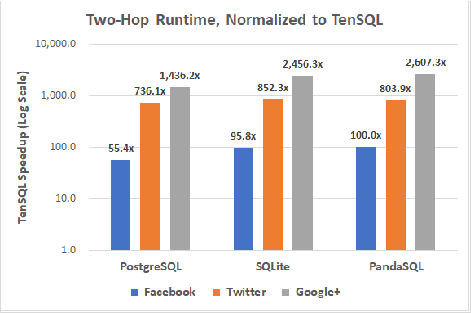
\includegraphics[width=0.45\textwidth]{pictures/tenSQL.pdf}};
\end{tikzpicture}
\end{frame}

\begin{frame}[fragile]
  \begin{center}
  \huge
  И всё было бы хорошо, но \ldots
  \end{center}
\end{frame}

\begin{frame}[fragile]
  \frametitle{Проблемы дизайна GraphBLAS\footnote{\href{https://docs.google.com/document/d/1fMmm-Bmew0wpgJRrjyMHy6G-zPq6R6kQlRum560_4S0/edit?tab=t.0}{What did GraphBLAS Get Wrong?}, John Gilbert, UC Santa Barbara, GraphBLAS BoF at HPEC, September 2022}}
  \begin{itemize}
    \item \ <<Естественная>> выразимость алгоритмов
    \begin{itemize}
      \item BFS vs DFS\footnote{\href{https://dl.acm.org/doi/10.1145/3315454.3329962}{Linear Algebraic Depth-First Search}}
    \end{itemize}
    \item Необходимы специфичные оптимизации
    \begin{itemize}
      \item Kernel Fusion для разреженных данных
      \item В целом, нерегулярный параллелизм --- это тяжело
    \end{itemize}  
    \item Неявные нули
    \item \ <<Громоздкость>> из-за ручных оптимизаций и необходимости тонких настроек    
    \item (Не)универсальность
    \item \ldots
  \end{itemize}
\end{frame}

\begin{frame}[fragile]
  \frametitle{Kernel Fusion}
  \begin{center}
    \[
    \underbrace{M_1 + M_2}_{M_4} + M_3 	\rightsquigarrow add(add(M_1,M_2), M_3)
    \]
  \end{center}
  \begin{itemize}
    \item[\faCheck] Stream Fusion --- для <<одномерных>> данных
    \item[\faCheck] XLA --- для плотных данных
    \item[\faGears] MLIR\footnote{Например, \href{https://mlir-graphblas.readthedocs.io/en/latest/}{mlir-graphblas}}
    \item[\faQuestion] Для разреженных вычислений в общем виде
    \begin{itemize}
      \item[\faFrownO] Для обобщённых вычислений
      \item[\faFrownO] Для GPGPU и других специализированных ускорителей
    \end{itemize}  
  \end{itemize}
\end{frame}

\begin{frame}[fragile]
  \frametitle{Неявные нули\footnote{\url{https://github.com/lessthanoptimal/ejml/pull/145\#issuecomment-888293732}}$^{,}$\footnote{\url{https://github.com/GraphBLAS/LAGraph/issues/28}}}
  \begin{itemize}
    \item Разреженный матрицы и вектора --- не храним <<нули>>
    \item C API --- сложно внятно описать на уровне типов, кто такие эти <<нули>>
    \begin{itemize}
      \item Часто появляются выделенные значения (<<давайте считать, что \texttt{0:Int} не храним>>)
      \item Пользовательские функции: не достаточно чёткие типы, сложно обрабатывать крайние случаи
      \item Переход между доменами: в одном домене выделенное значение не храним, а в другом должны хранить, потому что это <<значимый>> элемент, а выделенное значение другое
    \end{itemize}    
    \vfill
    \texttt{add (x:Int, y:Int):Int = x + y}
    \\ Можем получить 0. Должны сохранить?
  \end{itemize}
\end{frame}

\begin{frame}[fragile]
  \frametitle{<<Громоздкость>>}
  \begin{itemize}
    \item Ручное слияние ядер (kernel fusion) --- разрастается количество аргументов
    \begin{itemize}
      \item Маска --- аргумент умножения\footnote{$mask(M_1 * M_2, M_3) 	\rightsquigarrow mult(M_1,M_2,M_3)$}$^{,}$\footnote{Да, как \texttt{multiply\_add}} и не только
      \item Маска может быть инвертированной или нет      
    \end{itemize}
    \item Поэлементные операции
    \begin{itemize}
      \item \texttt{ewise\_add}, \texttt{ewise\_mult}, mask, \ldots\footnote{Почему не \texttt{map2} или что-то аналогичное? Отчасти, потому что проблема с нулями.}
    \end{itemize}
    \item Дескрипторы --- средство тонкой ручной настройки операций
    \item \ldots
  \end{itemize}
\end{frame}

\begin{frame}[fragile]
  \frametitle{(Не)универсальность}
  \begin{center}
    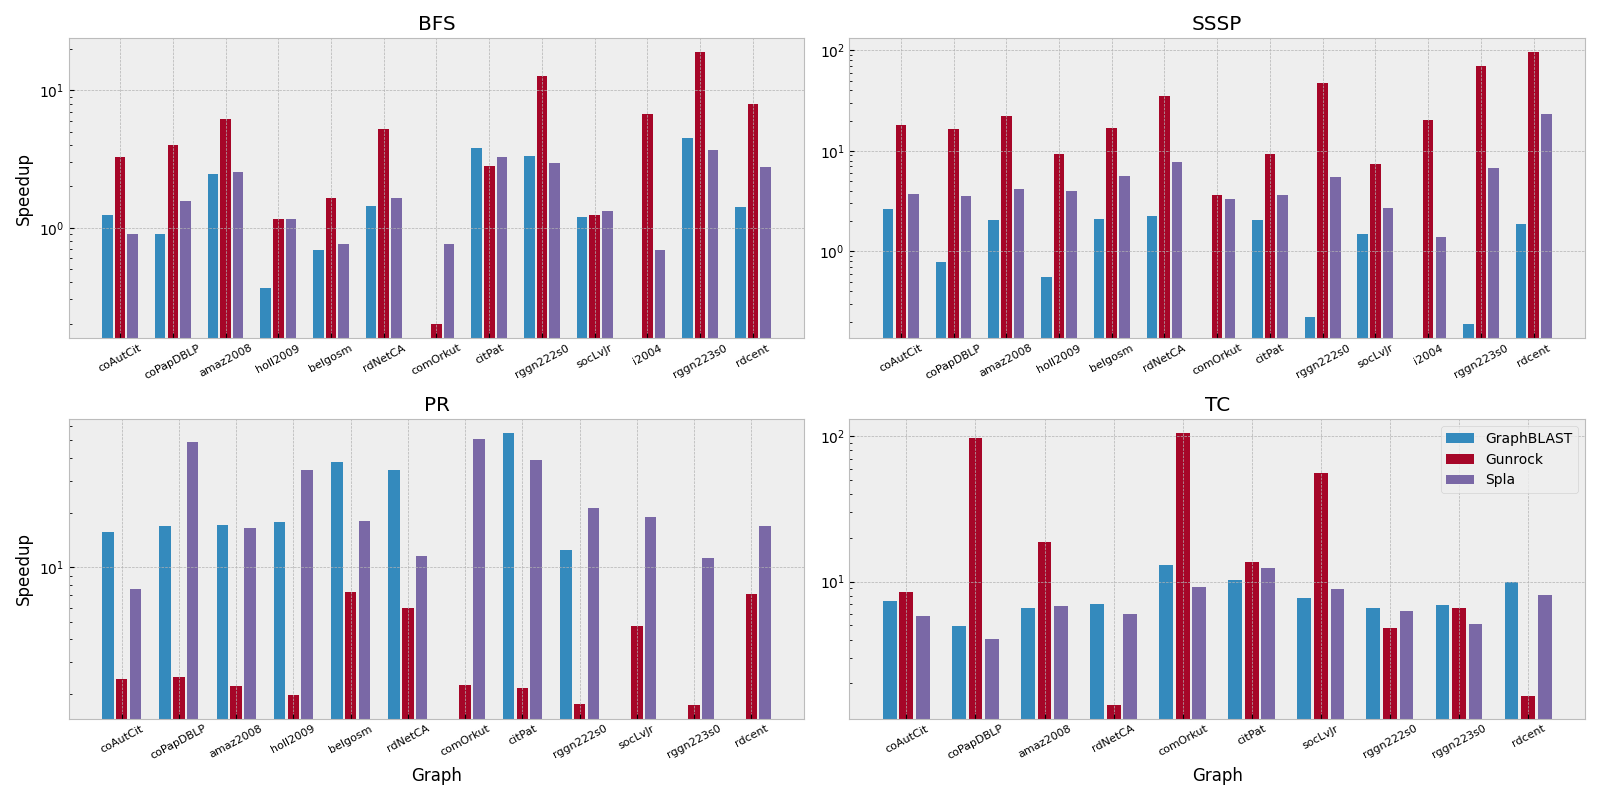
\includegraphics[width=0.85\textwidth]{pictures/rq1_rel.png}
  
  \scriptsize
  \begin{minipage}{0.49\textwidth}
  \begin{itemize}
  \item Ускорение относительно LAGraph 
  \item Графы из SuiteSparse Matrix Collection
  \end{itemize}
\end{minipage}
\begin{minipage}{0.49\textwidth}
  \begin{itemize}
  \item GraphBLAST и Spla --- GraphBLAS-подобные
  \item Gunrock --- BSP-like подход на основе BFS
  \end{itemize}
\end{minipage}
\end{center}  
\end{frame}

\begin{frame}[fragile]
  \frametitle{Выводы}
  \begin{itemize}
    \item Обобщённая разреженная линейная алгебра --- вполне рабочий инструмент высокопроизводительного анализа графов 
    \begin{itemize}
      \item FalkorDB, NetworkX, LAGraph, OneSparse, \ldots
    \end{itemize}
    \item Пока хорошо работает только на одном узле, in memory, многоядерные CPU
    \begin{itemize}
      \item SuiteSparse: GraphBLAS
    \end{itemize}
    \item Не лишён недостатков
    \begin{itemize}
      \item Если не пользуетесь готовыми прикладными алгоритмами, то думать о графах в терминах линейной алгебры --- отдельный навык
      \item Придумывать специальные полукольца и моноиды --- нетривиальное занятие
    \end{itemize}
  \end{itemize}
\end{frame}

\begin{frame}[fragile]
  \frametitle{Направления развития}
  \begin{itemize}
    \item Использование (специализированных) ускорителей
    \begin{itemize}
      \item В SuiteSparse:GraphBLAS ведётся работа по реализации некоторых ядер на Cuda
      \item Spla использует GPGPU через OpenCL 
    \end{itemize}
    \item Разработка специализированных ускорителей для разреженной линейной алгебры
    \begin{itemize}
      \item Расширения для RISC-V
      \item Более <<экзотические>> решения\footnote{\href{https://dl.acm.org/doi/10.1145/3640542}{Dedicated Hardware Accelerators for Processing of Sparse Matrices and Vectors: A Survey}}
    \end{itemize}
    \item Больше прикладных решений:
    анализ сетевого трафика\footnote{\href{https://catalog.caida.org/paper/2023_deployment_of_real_time_network_traffic_analysis_using_graphblas_hyperspace_matrices_and_d4m_associative_arrays}{Deployment of Real-Time Network Traffic Analysis Using GraphBLAS Hypersparse Matrices and D4M Associative Arrays}}, анализ кода\footnote{\href{https://dl.acm.org/doi/10.1145/3735544.3735585}{Universal High-Performance CFL-Reachability via Matrix Multiplication}}, \ldots
    \item Усовершенствование API 
    \begin{itemize}
      \item Ведётся работа над C++ API\footnote{\href{https://graphblas.org/graphblas-api-cpp/}{GraphBLAS C++ API Specification v1.0}} 
      \item Попытки применить идеи из функционального программирования\footnote{Алгебраические типы для работы <<нулями>>} 
    \end{itemize}
  \end{itemize}
\end{frame}

\appendix

\begin{frame}[t]
  \frametitle{Графы для экспериментов}
  \begin{center}
    \begin{table}[]
      \begin{tabular}{l|l|l|l|l|l}
      Name              & Vertices & Edges  & Avg Deg & Sd Deg & Max Deg  \\
      \hline\hline
      \rowcolor{Gray}
      coAuthorsCiteseer & 227.3K   & 1.6M   & 7.2     & 10.6   & 1372.0   \\
      coPapersDBLP      & 540.5K   & 30.5M  & 56.4    & 66.2   & 3299.0   \\
      \rowcolor{Gray}
      amazon-2008       & 735.3K   & 7.0M   & 9.6     & 7.6    & 1077.0   \\
      hollywood-2009    & 1.1M     & 112.8M & 98.9    & 271.9  & 11467.0  \\
      \rowcolor{Gray}
      belgium\_osm      & 1.4M     & 3.1M   & 2.2     & 0.5    & 10.0     \\
      roadNet-CA        & 2.0M     & 5.5M   & 2.8     & 1.0    & 12.0     \\
      \rowcolor{Gray}
      com-Orkut         & 3.1M     & 234.4M & 76.3    & 154.8  & 33313.0  \\
      cit-Patents       & 3.8M     & 33.0M  & 8.8     & 10.5   & 793.0    \\
      \rowcolor{Gray}
      rgg\_n\_2\_22\_s0 & 4.2M     & 60.7M  & 14.5    & 3.8    & 36.0     \\
      soc-LiveJournal   & 4.8M     & 85.7M  & 17.7    & 52.0   & 20333.0  \\
      \rowcolor{Gray}
      indochina-2004    & 7.4M     & 302.0M & 40.7    & 329.6  & 256425.0 \\
      rgg\_n\_2\_23\_s0 & 8.4M     & 127.0M & 15.1    & 3.9    & 40.0     \\
      \rowcolor{Gray}
      road\_central     & 14.1M    & 33.9M  & 2.4     & 0.9    & 8.0     
      \end{tabular}
    \end{table}
  \end{center}
\end{frame}


\begin{frame}[fragile]
  \frametitle{Пример: обход в ширину}
  \begin{minipage}{0.2\textwidth}
  \begin{tikzpicture}[shorten >=1pt,auto]
    \node[state] (q_0)                      {$0$};
    \node[state] (q_1) [above right=of q_0] {$1$};
    \node[state,fill=red!20] (q_2) [right=of q_0]       {$2$};
    \node[state] (q_3) [right=of q_2]       {$3$};
    \path[->]
    (q_0) edge  node {} (q_1)
    (q_1) edge  node {} (q_2)
    (q_2) edge  node {} (q_0)
    (q_2) edge[bend left, above]  node {} (q_3)
    (q_3) edge[bend left, below]  node {} (q_2);
    \end{tikzpicture}
  \end{minipage}~\pause
  \tikzmark{xPos}{}
  \begin{minipage}{0.75\textwidth}    
    \begin{equation*}
      \left(\begin{array}{cccc}        
        0  & 0  & \colR 1 & 0 \\        
      \end{array}\right)
      \times    
      \left(\begin{array}{cccc}        
        0 & 1 & 0 & 0 \\
        0 & 0 & 1 & 0 \\
        \rowcolor{red!20}
        1 & 0 & 0 & 1 \\
        0 & 0 & 1 & 0 \\        
      \end{array}\right)
      =      
        \left(\begin{array}{cccc}        
          \colB 1 & 0  & 0 & \colB 1 \\        
        \end{array}\right)
    \end{equation*}
    \mycallout<2-4>[opacity=1]{$(xPos) + (2.9,0.4)$}{Текущий фронт}{2.5}
    \mycallout<2-4>[opacity=1]{$(xPos) + (5.9,1.1)$}{Матрица смежности}{3.5}
    \mycallout<2-4>[opacity=1]{$(xPos) + (9.2,0.4)$}{Новый фронт}{2.5}
    \mycalloutR<2-4>[opacity=1]{$(xPos) + (4.3,0.2)$}{Полукольцо}{2.1}
  \end{minipage}

  \pause

  \begin{minipage}{0.2\textwidth}
    \begin{tikzpicture}[shorten >=1pt,auto]
      \node[state, fill=blue!20] (q_0)                      {$0$};
      \node[state] (q_1) [above right=of q_0] {$1$};
      \node[state, fill=red!20] (q_2) [right=of q_0]       {$2$};
      \node[state, fill=blue!20] (q_3) [right=of q_2]       {$3$};
      \path[->]
      (q_0) edge  node {} (q_1)
      (q_1) edge  node {} (q_2)
      (q_2) edge  node {} (q_0)
      (q_2) edge[bend left, above]  node {} (q_3)
      (q_3) edge[bend left, below]  node {} (q_2);
      \end{tikzpicture}
    \end{minipage}~
    \begin{minipage}{0.75\textwidth}
    \begin{equation*}
      \left(\begin{array}{cccc}        
        \colB 1 & 0  & 0 & \colB 1 \\        
      \end{array}\right)
      \times
      \left(\begin{array}{cccc}        
        \rowcolor{blue!20}
        0 & 1 & 0 & 0 \\
        0 & 0 & 1 & 0 \\        
        1 & 0 & 0 & 1 \\
        \rowcolor{blue!20}
        0 & 0 & 1 & 0 \\        
      \end{array}\right)
      =      
        \left(\begin{array}{cccc}        
          0 & \colG 1  & \colG 1 & 0 \\        
        \end{array}\right)
    \end{equation*}
    \pause     
    \begin{tikzpicture}[overlay,remember picture,auto]
        \draw (9.16, 1.21) node[cross=10pt, color=red] {};
    \end{tikzpicture}
  \end{minipage}

\end{frame}


\end{document}
